% Drawing 119/08-10 -- folder 119, batch 08, archive page 156 (PDF page 157).
% Transcription: deux triangles hachurés
% Kind: two hatched triangles. Method 2 (schematic redraw from the facsimile). Status: partial.
% Notes: Two hatched triangles side by side: a long one with its apex at the left (vertices A, B at the top, C at the bottom right, each edge drawn between the same vertices) and a smaller one to its right (D, E, F), the dotted vertices thickened as on the page; a thin line runs from the apex A to the left vertex D of the second triangle. His hatching is a zigzag; it is drawn as a regular hatch. Still differs: a stroke from the top vertex B to a dot at the upper right (before the words "ce"), and a faint stroke from there towards E, which may close a third triangle B-dot-E, are left out as uncertain; the struck/overwritten letters on the left half of the first triangle are left out. Redrawn 2026-11-09 (issue 128): to check again. Question settled by a machine pass on the facsimile, 2026-11-12 (page): at 700 dpi a solid stroke runs from the top vertex B to a full dot at the upper right, before the word « ce », and a thin stroke runs from near B to the top vertex E of the second triangle; no stroke joins the dot to E, so there is no third closed triangle. Both strokes and the dot are now drawn (the thin one in pencil). Not checked by a reader.
% Coordinates: 1 unit = 1 mm = 1/100 of the crop width (bbox in page fractions: [0.72, 0.515, 0.86, 0.565]).
% Redrawn by Claude (claude-opus-5-5), issue #73, 2026-11-09; not checked by a human; not compiled (no TeX in the session).
% Rights: reproduces part of the work -- behind RENDER_TRANSCRIPTS, never published by itself.
\documentclass[tikz,border=3pt]{standalone}
\usepackage{amsmath,amssymb}
\usetikzlibrary{patterns,arrows.meta}
\tikzset{pencil/.style={black!45}, struck/.style={black!35}, mark/.style={circle,draw,inner sep=1.3pt}, pt/.style={circle,fill,inner sep=0.9pt}, opt/.style={circle,draw,fill=white,inner sep=1.1pt}}
\begin{document}
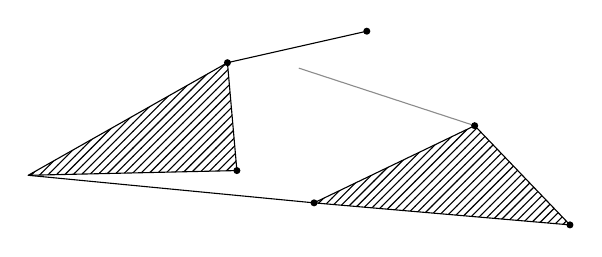
\begin{tikzpicture}[x=1mm,y=1mm,line cap=round,line join=round,font=\scriptsize]
\fill[pattern=north east lines] (17.8,-27.1) -- (43.1,-12.8) -- (44.3,-26.5) -- cycle;
\draw (17.8,-27.1) -- (43.1,-12.8) -- (44.3,-26.5) -- cycle;
\fill[pattern=north east lines] (54.1,-30.6) -- (74.5,-20.8) -- (86.6,-33.4) -- cycle;
\draw (54.1,-30.6) -- (74.5,-20.8) -- (86.6,-33.4) -- cycle;
\draw (17.8,-27.1) -- (54.1,-30.6);
\draw (43.1,-12.8) -- (60.8,-8.8);
\draw[pencil] (52.2,-13.5) -- (74.5,-20.8);
\node[pt] at (43.1,-12.8) {};
\node[pt] at (60.8,-8.8) {};
\node[pt] at (44.3,-26.5) {};
\node[pt] at (54.1,-30.6) {};
\node[pt] at (74.5,-20.8) {};
\node[pt] at (86.6,-33.4) {};
\end{tikzpicture}
\end{document}
